In this chapter, we present two demos that explore the high-level and safety 
capabilities of \CEU described in the previous chapter.
%
Our goal is to present full commented applications that help understanding and 
getting familiar with the language.
%
The applications are somewhat simple (70 and 170 lines), but complete enough to 
expose the programming techniques promoted by \CEU.

The first demo targets commercially available 16-bit WSN nodes, such as 
\emph{micaZ} and \emph{telosb}%
\footnote{\url{http://www.xbow.com}}.
The second demo uses the Arduino open-source platform%
\footnote{\url{http://arduino.cc}}, in order to experiment with custom
third-party hardware.
Both platforms have low processing power and memory capacity (16Mhz CPU, 32Kb 
Flash, and 4Kb SRAM), showing that \CEU is applicable to highly constrained 
platforms.

\section{WSN ring}
\label{sec:demos:ring}

In the first demo, we implement a fixed-ring topology with $N$ motes placed 
side-by-side which should all follow the same behavior: receive a message with 
an integer counter, show it on the LEDs, wait for $1$ second, increment the 
counter, and forward it to the mote on its right.
%Note that using fixed topologies and running the same application in all motes 
%are common practices in the context of WSNs.
%
Because the topology constitutes a ring, the counter will be incremented 
forever while traversing the motes.
%
If a mote does not receive a message within $5$ seconds, it should blink the 
red LED every $500$ milliseconds until a new message is received.
%In a ring topology, communications traverse all motes, and the network goes 
%down with a failure in a single mote, making tests much easier.
%
The mote with \emph{id=0} is responsible for initiating the process at boot 
time and recovering the ring from failures.
On perceiving a failure, it should wait for $10$ seconds before retrying the 
communication.

\begin{figure}[ht]
\begin{lstlisting}[numbers=left,xleftmargin=2em]
loop do
    var _message_t* msg = await RADIO_RECEIVE;
    var int* cnt = _Radio_getPayload(msg);
    _Leds_set(*cnt);
    await 1s;
    *cnt = *cnt + 1;
    finalize
        _Radio_send((_NODE_ID+1)%N, msg);
    with
        _Radio_cancel(msg);
    end
    await RADIO_SENDDONE;
end
\end{lstlisting}
\rule{14cm}{0.37pt}
\caption{ Communicating trail for the WSN ring.%\newline
{\small %\textmd{
%The code is a simple loop that does not handle failures.
}%}
\label{lst.ring.1}
}
\end{figure}

Figure~\ref{lst.ring.1} implements the communicating trail, which continuously 
receives and forwards the messages.
%
The code is an endless loop that first awaits a radio message (line 2), gets a 
pointer to its data buffer (line 3), shows the received counter on the LEDs 
(line 4), and then awaits $1$s (line 5) before incrementing the counter in the 
message (line 6) and forwarding it to the next mote (line 7-12).

The program uses several services provided by the underlying operating system 
(\cite{wsn.tos}), which are all non-blocking $C$ functions for LEDs and radio 
manipulation.

The finalization block (lines 7-11) ensures that regardless of how the 
communicating trail is composed with the rest of the application (and 
eventually aborted by it), the \code{msg} buffer will be safely released while 
waiting for a \code{RADIO\_SENDDONE} acknowledge from the radio driver.

Because this code does not handle failures, it is straight to the point and 
easy to follow.
Actually, this is the final code for this task, as error handling is placed in 
a parallel trail.

\begin{comment}
Note that the program accesses the message buffer multiple times in reaction to 
events.
However, given that the \code{await} primitive provides sequential flow across 
reactions to events, every access to the buffer in the code is undoubtedly 
deterministic.
In typical event-driven systems~\cite{wsn.nesc}, the accesses would be split in 
multiple callbacks, requiring a thoughtful reasoning about concurrency issues.
\end{comment}

\begin{figure}[ht]
\begin{lstlisting}[numbers=left,xleftmargin=2em]
par do
    <...> // COMMUNICATING TRAIL (previous code)
with
    loop do
        par/or do
            await RADIO_RECEIVE;
        with
            await 5s;
            par do
                loop do
                    emit retry; // only captured by mote 0
                    await 10s;
                end
            with
                _Leds_set(0);   // clear LEDs
                loop do
                    _Leds_led0Toggle();
                    await 500ms;
                end
            end
        end
    end
end
\end{lstlisting}
\rule{14cm}{0.37pt}
\caption{ Monitoring trail for the WSN ring.%\newline
{\small %\textmd{
%The code is a simple loop that does not handle failures.
}%}
\label{lst.ring.2}
}
\end{figure}

To handle failures, we define in Figure~\ref{lst.ring.2} a monitoring trail 
(lines 4-22) in parallel with the communicating trail.
%
Lines 8 to 20 describe the network-down behavior.
After $5$ seconds of inactivity are detected in the sub-trails in parallel 
(lines 6 and 8), two new activities run in parallel: one that retries 
communication every $10$ seconds by signaling the internal event \code{retry} 
(lines 8-11); and another that blinks the red LED every $500$ milliseconds 
(lines 13-17).

The trick to restore the normal behavior of the network is to await event 
\code{RADIO\_RECEIVE} (line 6) in the \code{par/or} (line 5) with the 
network-down behavior to abort it whenever a new message is received.
By surrounding everything with a \code{loop} (line 4), we ensure that the error 
detection is continuous.

\begin{figure}[ht]
\begin{lstlisting}[numbers=left,xleftmargin=2em]
par do
    <...> // COMMUNICATING TRAIL
with
    <...> // MONITORING TRAIL
with
    if _NODE_ID == 0 then
        loop do
            var _message_t msg;
            var int* cnt = _Radio_getPayload(&msg);
            *cnt = 1;
            finalize
                _Radio_send(1, &msg);
            with
                _Radio_cancel(&msg);
            end
            await retry;
        end
    else
        await FOREVER;
    end
end
\end{lstlisting}
\rule{14cm}{0.37pt}
\caption{ Retrying trail for the WSN ring.%\newline
{\small %\textmd{
%The code is a simple loop that does not handle failures.
}%}
\label{lst.ring.3}
}
\end{figure}

Finally, we implement in Figure~\ref{lst.ring.3} the initiating/retrying 
process that sends the first message from mote with \emph{id=0}.
Again, we place the code (lines 6-20) in parallel with the other activities.
%
As this process is only handled by the mote with $id=0$, we start by checking 
it (line 6).
If this is not the case, we simply await forever on this trail (line 19).
Otherwise, the \code{loop} (lines 7-17) sends the first message as soon as the 
mote is turned on (line 12).
It then waits for a \code{retry} emit (line 16) to loop and resend the initial 
message.
Remind that event \code{retry} is emitted on network-down every $10$ seconds 
(line 10 of Figure~\ref{lst.ring.2}).

The static analysis of \CEU correctly warns about concurrent calls to 
\code{\_Radio\_send} (line 12) \emph{vs.} \code{\_Leds\_set} and 
\code{\_Leds\_led0Toggle} (lines 15,17 of Figure~\ref{lst.ring.2}), which all 
execute after the program detects 5 seconds of inactivity (line 6 of 
Figure~\ref{lst.ring.2}).
However, because these functions affect different devices (i.e. radio 
\emph{vs.} LEDs), they can be safely executed concurrently.
The following annotation (to be included in the program) states that these 
specific functions can be called concurrently with deterministic behavior, 
allowing the program to be compiled without warnings:

\begin{lstlisting}
  safe _Radio_send with
       _Leds_set, _Leds_led0Toggle;
\end{lstlisting}

This example shows how complementary activities in an application can be 
written in separate and need not to be mixed in the code.
In particular, error handling (monitoring trail) need not interfere with 
regular behavior (communicating trail), and can even be incorporated later.
To ensure that parallel activities exhibit deterministic behavior, the \CEU 
compiler rejects harmful concurrent $C$ calls by default.

\begin{figure}[ht]
\begin{lstlisting}[numbers=left,xleftmargin=2em]
input int SWITCH;
var int cur_app = 1;
loop do
    par/or do
        cur_app = await SWITCH;
    with
        if cur_app == 1 then
            <...>  // CODE for APP1
        end
        if cur_app == 2 then
            <...>  // CODE for APP2
        end
        await FOREVER;
    end
end
\end{lstlisting}
\rule{14cm}{0.37pt}
\caption{ Retrying trail for the WSN ring.%\newline
{\small %\textmd{
%The code is a simple loop that does not handle failures.
}%}
\label{lst.app}
}
\end{figure}

As a final consideration, we can extend the idea of compositions by combining 
different \emph{applications} together.
In the context of WSNs, it is usually difficult to physically recover motes in 
a deployed network, and by combining multiple applications in a single image, 
we can switch their execution remotely via radio.
%
The archetype in Figure~\ref{lst.app} illustrates this idea.
%
The input event \code{SWITCH} (line 1) is used to request application switches 
remotely.%
\footnote{ We are assuming the existence of an hypothetical high-level event 
\code{SWITCH} that abstracts the radio protocol for requests to change the 
current running application. }
Initially, the code behaves as application $1$ (lines 7-9), but is also waiting 
for a \code{SWITCH} request in parallel (line 5).
Whenever a new request occurs, the \code{par/or} terminates, aborts the running 
application, and restarts as the requested application.
The statement \code{await FOREVER} (line 13) ensures that a terminating 
application does not reach the end of the \code{par/or} and restarts itself.

The same idea can be used to \emph{reboot} a mote remotely, in the case of a 
strange behavior in an application.

\section{Spaceship game}

In the next demo, a spaceship game, we control a ship that moves through space 
and has to avoid collisions with meteors until it reaches the finish line.
%
Although this application is not networked, it is still embedded and reactive, 
using timers, buttons, and an LCD with real-time feedback.
%
We use an Arduino connected to a third-party two-row LCD display with two 
buttons to exhibit and control the spaceship.
%
Figure~\ref{fig:ship} shows the picture of a running quest.

\begin{figure}[t]
\centering
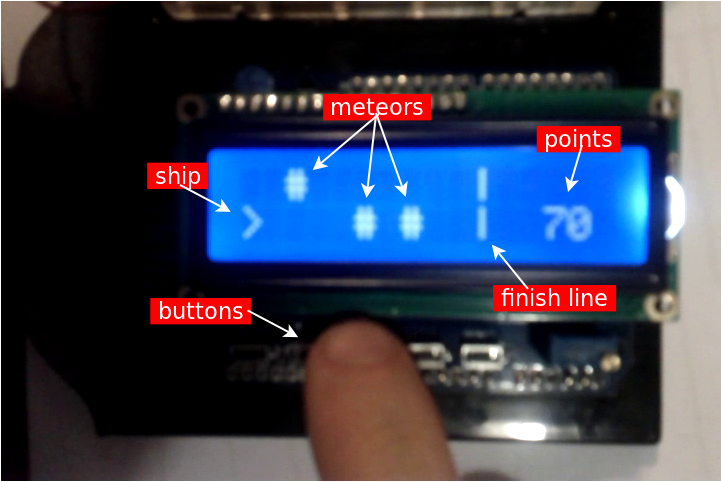
\includegraphics[scale=0.30]{ship.png}
\caption{ The ``spaceship'' game
\label{fig:ship}
}
\end{figure}

\begin{figure}[ht]
\begin{lstlisting}[numbers=left,xleftmargin=2em]
var int dt;       // inverse of game speed
var int points;   // number of steps alive
var int win = 0;  // starting the game

loop do
    <...> // CODE 1: set game attributes

    _map_generate();
    _redraw(x, y, points);
    await KEY;  // starting key

    <...> // CODE 2: the central loop

    <...> // CODE 3: game over
end
\end{lstlisting}
\rule{14cm}{0.37pt}
\caption{ Outermost loop for the game.
{\small %\textmd{
%The code is a simple loop that does not handle failures.
}%}
\label{lst.ship.1}
}
\end{figure}

We describe the behavior of the game, along with its implementation, following 
a top-down approach.
The outermost loop of the game, in Figure~\ref{lst.ship.1}, is constituted of 
\code{CODE~1}, which sets the game attributes such as globals \code{code} and 
\code{dt}; \code{CODE~2} with the central game loop; and \code{CODE~3} with the 
``game over'' animation.
%
Every time the loop is executed, it resets the game attributes (line 5), 
generates a new map (line 7), redraws it on screen (line 8), and waits for a 
starting key (line 9).
Then, the program executes the main logic of the game (line 11), until the 
spaceship reaches the finish line or collides with a meteor.
Depending on the result held in \code{win}, the ``game over'' code (line 13) 
may display an animation before restarting the game.

\begin{figure}[ht]
\begin{lstlisting}[numbers=left,xleftmargin=2em]
    // CODE 1: set game attributes
    var int y = 0;          // ship coordinates
    var int x = 0;          //  restart every phase

    if not win then
        dt     = 500;
        points = 0;
    else
        if dt > 100 then
            dt = dt - 50;
        end
    end
\end{lstlisting}
\rule{14cm}{0.37pt}
\caption{ Sets the game attributes.
{\small %\textmd{
%The code is a simple loop that does not handle failures.
}%}
\label{lst.ship.2}
}
\end{figure}

The game attributes (\code{CODE 1} in Figure~\ref{lst.ship.2}) change depending 
on the result of the previous iteration of the outermost loop.
%
For the first game execution and whenever the spaceship collides with a meteor, 
variable \code{win} is false, hence, the attributes are reset to their initial 
values (lines 6-7)
Otherwise, if the player reached the finish line, then the game gets faster, 
keeping the current points (lines 9-11).

\begin{figure}[ht]
\begin{lstlisting}[numbers=left,xleftmargin=2em]
    // CODE 2: the central loop
    par/or do
        loop do
            await (dt)ms;
            x = x + 1;
            _redraw(x, y, points);

            if _MAP[y][x] == '#' then
                win = 0;  // a collision
                break;
            end

            if x == _FINISH then
                win = 1;  // finish line
                break;
            end

            points = points + 1;
        end
    with
        loop do
            var int key = await KEY;
            if key == _KEY_UP then
                y = 0;
            end
            if key == _KEY_DOWN then
                y = 1;
            end
        end
    end;
\end{lstlisting}
\caption{ The game central loop.
{\small %\textmd{
%The code is a simple loop that does not handle failures.
}%}
\label{lst.ship.3}
}
\end{figure}

The central loop of the game (\code{CODE 2}  in Figure~\ref{lst.ship.3}) moves 
the spaceship as time elapses and checks whether the spaceship reaches the 
finish line or collides with a meteor.
%
The code is actually split in two loops in parallel: one that runs the game 
steps (lines 3-19), and the other that handles input from the player to move 
the spaceship (lines 21-29).
Note that we want the spaceship to move only during the game action, this is 
why we did not place the input handling in parallel with the whole application.

The game steps run periodically, depending on the current speed of the game 
(line 4).
For each loop iteration, \code{x} is incremented and the current state is 
redrawn on screen (lines 5-6).
Then, the spaceship is checked for collision with meteors (lines 8-11), and 
also with the finish line (lines 13-16).
In either of the cases, the central loop terminates with \code{win} set to the 
proper value, also canceling the input handling activity.
The points are incremented before each iteration of the loop (line 18).

To handle input events, we wait for key presses in another loop (line 22) and 
change the spaceship position accordingly (lines 24, 27).
Note that there are no possible race conditions on variable \code{y} (i.e., 
lines 6,8 \emph{vs.} 24,27) because the two loops in the \code{par/or} 
statement react to different events (i.e., time and key presses).

\begin{figure}[ht]
\begin{lstlisting}[numbers=left,xleftmargin=2em]
    // CODE 3: game over
    par/or do
        await KEY;
    with
        if !win then
            loop do
                await 100ms;
                _lcd.setCursor(0, y);
                _lcd.write('<');
                await 100ms;
                _lcd.setCursor(0, y);
                _lcd.write('>');
            end
        end
    end
\end{lstlisting}
\caption{ The ``game over'' behavior for the game.
{\small %\textmd{
%The code is a simple loop that does not handle failures.
}%}
\label{lst.ship.4}
}
\end{figure}

After escaping the central loop, we run the code of Figure~\ref{lst.ship.4} for 
the ``game over'' behavior, which starts an animation if the spaceship collides 
with a meteor.
%
The animation loop (lines 6-13) continuously displays the spaceship in the two 
directions, suggesting that it has hit a meteor.
The animation is interrupted when the player presses a key (line 3), proceeding 
to the game restart.
Note the use of the \code{\_lcd} object, available in a third-party \emph{C++} 
library shipped with the LCD display.%, and used unmodified in the example.

This demo makes extensive use of global variables, relying on the
deterministic concurrency analysis guaranteed by the \CEU compiler.
We used a top-down approach to illustrate the hierarchical compositions of 
blocks of code.
For instance, the ``game over'' animation (lines 6-13) is self-contained and 
can be easily adapted to a new behavior without considering the other parts of 
the program.
